\section{Implémentation et statistique}
L'implémentation sera diviser en deux partie la première consiste à lancer le programme en variant le nombre des fourmis ($\mathtt{\sim}\ nbAnts $) à chaque fois qu'on passe les $ m $ exécution ($ m \mathtt{\sim}\ exec $) et la deuxième partie consiste à fixer le nombre des fourmis et interpréter les statistique les différentes  problèmes qu'on a.

%expereience 1
\flushleft

\subsection{Expérience 1}
Les résultats de Greedy appliquer sur cities.dat, cities2.dat .
\subsection*{ \centering Exp. 3 on cities.dat \comm{figure of PathofGcities cities of exp 2}}

\begin{figure}[H]
	\begin{minipage}[t]{0.45\linewidth}
	\centering
	\includegraphics[width=\textwidth]{\PathofGcities/path.eps}
	\caption{Path journey and Totale distance}\label{fig:PathofGcities:path}
	
	\end{minipage}\hfill
	\begin{minipage}[t]{0.45\linewidth}
	\centering
	\includegraphics[width=\textwidth]{\PathofGcities/ExecTimeAndMeanSTDWith.eps}
	\caption{Execution Time and Mean and STD on cities.dat}
	\label{fig:PathofGcities:AS_1_5AS_ExecTimeAndMeanSTDWith_execVariation}
	\end{minipage}
\end{figure}

\subsection*{ \centering Exp. 3 on cities2.dat \comm{figure of PathofGcitiesdeux cities2 of exp 3}}
\begin{figure}[H]
	\begin{minipage}[t]{0.45\linewidth}
	\centering
	\includegraphics[width=\textwidth]{\PathofGcitiesdeux/path.eps}
	\caption{Path journey and Totale distance}\label{fig:PathofGcitiesdeux:path}
	
	\end{minipage}\hfill
	\begin{minipage}[t]{0.45\linewidth}
	\centering
	\includegraphics[width=\textwidth]{\PathofGcitiesdeux/ExecTimeAndMeanSTDWith.eps}
	\caption{Execution Time and Mean and STD on cities2.dat}
	\label{fig:PathofGcitiesdeux:AS_1_5AS_ExecTimeAndMeanSTDWith_execVariation}
	\end{minipage}
\end{figure}
\comm{}
\subsection*{ \centering Exp. 3 on rand 50.dat\comm{figure of PathofGcinq of exp 3}}
\begin{figure}[H]
	\begin{minipage}[t]{0.45\linewidth}
	\centering
	\includegraphics[width=\textwidth]{\PathofGcinq/path.eps}
	\caption{Path journey and Totale distance}\label{fig:PathofGcinq:path}
	
	\end{minipage}\hfill
	\begin{minipage}[t]{0.45\linewidth}
	\centering
	\includegraphics[width=\textwidth]{\PathofGcinq/ExecTimeAndMeanSTDWith.eps}
	\caption{Execution Time and Mean and STD on rand50.dat}
	\label{fig:PathofGcinq:AS_1_5AS_ExecTimeAndMeanSTDWith_execVariation}
	\end{minipage}
\end{figure}

\subsection*{ \centering Exp. 3 on rand 60.dat\comm{figure of PathofGsix of exp 2}}
\begin{figure}[H]
	\begin{minipage}[t]{0.45\linewidth}
	\centering
	\includegraphics[width=\textwidth]{\PathofGsix/path.eps}
	\caption{Path journey and Totale distance}\label{fig:PathofGsix:path}
	
	\end{minipage}\hfill
	\begin{minipage}[t]{0.45\linewidth}
	\centering
	\includegraphics[width=\textwidth]{\PathofGsix/ExecTimeAndMeanSTDWith.eps}
	\caption{Execution Time and Mean and STD on rand60.dat}
	\label{fig:PathofGsix:AS_1_5AS_ExecTimeAndMeanSTDWith_execVariation}
	\end{minipage}
\end{figure}


\subsection*{ \centering Exp. 3 on rand 80.dat\comm{figure of PathofGhuit of exp 3}}
\begin{figure}[H]
	\begin{minipage}[t]{0.45\linewidth}
	\centering
	\includegraphics[width=\textwidth]{\PathofGhuit/path.eps}
	\caption{Path journey and Totale distance}\label{fig:PathofGhuit:path}
	
	\end{minipage}\hfill
	\begin{minipage}[t]{0.45\linewidth}
	\centering
	\includegraphics[width=\textwidth]{\PathofGhuit/ExecTimeAndMeanSTDWith.eps}
	\caption{Execution Time and Mean and STD on rand50.dat}
	\label{fig:PathofGhuit:AS_1_5AS_ExecTimeAndMeanSTDWith_execVariation}
	\end{minipage}
\end{figure}

\subsection*{ \centering Exp. 3 on rand 100.dat\comm{figure of PathofGcent of exp 3}}

\begin{figure}[H]
	\begin{minipage}[t]{0.45\linewidth}
	\centering
	\includegraphics[width=\textwidth]{\PathofGcent/path.eps}
	\caption{Path journey and Totale distance}\label{fig:PathofGcent:path}
	
	\end{minipage}\hfill
	\begin{minipage}[t]{0.45\linewidth}
	\centering
	\includegraphics[width=\textwidth]{\PathofGcent/ExecTimeAndMeanSTDWith.eps}
	\caption{Execution Time and Mean and STD on rand50.dat}
	\label{fig:PathofGcent:AS_1_5AS_ExecTimeAndMeanSTDWith_execVariation}
	\end{minipage}
\end{figure}
\comm{}

On peut voir clairement que le \textit{\textbf{Greedy}} ne donne pas des bonnes résultats par rapport à \textbf{\textit{AS}} ou même par rapport à \textit{\textbf{SA}} la distance totale dans Greedy est beaucoup plus grands, si on regarde par exemple la figure \ref{fig:Pathofcities:path} la distance $ \simeq 27.51$  alors que dans Greedy la distance totale $ \simeq 53.26$ \ref{fig:PathofGcities:path} mais c'est à prix de temps le temps d'exécution en Greedy  $\simeq 0.1733$  alors qu'il augmente dans le AS pour arriver à un moyenne de  0.542 et en moyenne Greedy $ \simeq 0.015 $ et AS $ \simeq 0.542$.

\subsection{Expérience 2}
Les résultats ci-dessous sont sur la première expérience ou je lance le programme en variant le nombre des fourmis, l'expérience est fait sur les fichiers suivants 
\textcolor{blue}{cities.dat},  \textcolor{blue}{cities2.dat},  \textcolor{blue}{rand50.dat} et  \textcolor{blue}{rand100.dat} en variant le nombre des fourmis.
\comm{figures of result of executions experiments 1 on cities, cities2, rand50 and rand100 with n variation}

\subsection*{ \centering Exp. 1 on cities.dat \comm{PathofcitiesNvariation of exp1}}
\begin{figure}[H]
	\begin{minipage}[t]{0.5\linewidth}
		\includegraphics[width=\linewidth]{\PathofcitiesNvariation/path.eps}
		\caption{Path journey}
		\label{fig:PathofcitiesNvariation:path}
	\end{minipage}
	\hspace{2mm}
	\begin{minipage}[t]{0.5\linewidth}
	\includegraphics[width=\linewidth]{\PathofcitiesNvariation/AS_1_5AS_ExecTimeAndMeanSTDWith_execVariation.eps}
	\caption{Variation of the execution time VS the \# of ants (20$\stackrel{step=20}{\rightarrow}$100) in each execution (1$\stackrel{step=1}{\rightarrow}$ 5)}
	\label{fig:PathofcitiesNvariation:AS_1_5AS_ExecTimeAndMeanSTDWith_execVariation}
	\end{minipage}
\end{figure}
\begin{figure}[H]
		\begin{minipage}[t]{.5\linewidth}
		\centering
		\includegraphics[width=\linewidth]{\PathofcitiesNvariation/AS_BestCost_Varying_Iteration_and_nbAnts.eps}
		\caption{Best cost VS Ants number variation with $\alpha$=1, $ \beta $ = 5}
		\label{fig:PathofcitiesNvariation:AS_BestCost_Varying_Iteration_and_nbAnts}
		\end{minipage}
		\begin{minipage}[t]{.5\linewidth}
		\includegraphics[width=\linewidth]{\PathofcitiesNvariation/AS15ExecAcheivingBestCost.eps}
		\caption{AS15ExecAcheivingBestCost $\alpha$=1, $ \beta $ = 5}
		\label{fig:PathofcitiesNvariation:AS15ExecAcheivingBestCost}
		\end{minipage}
\end{figure}
% % % %
	\begin{minipage}[t]{0.9\linewidth}
	\vspace{-10mm}
	\begin{table}[H]
	\label{tab:PathofcitiesNvariation:expdeux}
	\begin{tabular}{lllll}
	\cline{1-2}
	\multicolumn{1}{|l|}{Best Costs results for experience 2 on cities.dat }                                                           &  \multicolumn{1}{l|}{Elapsed Time, Mean, STD}                                             &  &  &  \\ \cline{1-2}
	\multicolumn{1}{|l|}{\begin{tiny}\begin{tabular}{|l|c|c|c|c|c|c|c|c|c|c|}
\hline
&\textbf{It :1}&\textbf{It :2}&\textbf{It :3}&\textbf{It :4}&\textbf{It :5}&\textbf{It :6}&\textbf{It :7}&\textbf{It :8}&\textbf{It :9}&\textbf{It :10}\\\hline
\textbf{exec :1}&28.07&28.07&28.07&28.07&28.07&28.07&28.07&27.52&27.52&27.52\\\hline
\textbf{exec :2}&28.86&28.86&28.86&28.86&28.86&28.86&27.52&27.52&27.52&27.52\\\hline
\textbf{exec :3}&29.16&29.13&28.05&28.05&28.05&28.05&28.05&28.05&27.72&27.52\\\hline
\textbf{exec :4}&29.05&27.52&27.52&27.52&27.52&27.52&27.52&27.52&27.52&27.52\\\hline
\textbf{exec :5}&29.47&27.52&27.52&27.52&27.52&27.52&27.52&27.52&27.52&27.52\\\hline
\textbf{exec :6}&28.66&28.09&27.52&27.52&27.52&27.52&27.52&27.52&27.52&27.52\\\hline
\textbf{exec :7}&28.05&27.72&27.52&27.52&27.52&27.52&27.52&27.52&27.52&27.52\\\hline
\textbf{exec :8}&27.72&27.52&27.52&27.52&27.52&27.52&27.52&27.52&27.52&27.52\\\hline
\textbf{exec :9}&27.52&27.52&27.52&27.52&27.52&27.52&27.52&27.52&27.52&27.52\\\hline
\textbf{exec :10}&27.52&27.52&27.52&27.52&27.52&27.52&27.52&27.52&27.52&27.52\\\hline
\end{tabular}
\end{tiny}} & \multicolumn{1}{l|}{\begin{tiny}\begin{tabular}{|l|c|}
\hline
&\textbf{Elapsed time}\\\hline
\textbf{exec :1}&0.29\\\hline
\textbf{exec :2}&0.54\\\hline
\textbf{exec :3}&0.78\\\hline
\textbf{exec :4}&1.02\\\hline
\textbf{exec :5}&1.27\\\hline
\textbf{exec :6}&2.48\\\hline
\textbf{exec :7}&3.73\\\hline
\textbf{exec :8}&4.96\\\hline
\textbf{exec :9}&6.16\\\hline
\textbf{exec :10}&12.40\\\hline
\textbf{ Mean}&3.36\\\hline
\textbf{ STD}&3.75\\\hline
\end{tabular}
\end{tiny} } &  &  &  \\ \cline{1-2}
	&     &  &  &  \\
	&     &  &  & 
	\end{tabular}
	\caption{Results of experience 2 on cities.dat}
	\end{table}
	\end{minipage}
% %

\subsection*{ \centering Exp. 1 on cities2.dat \comm{ResultOfcitiesDEUXNvariation of exp 1}}
	\vspace{-6mm}
\begin{figure}[H]
	\begin{minipage}[t]{0.5\linewidth}
		\includegraphics[width=\linewidth]{\ResultOfcitiesDEUXNvariation/path.eps}
		\caption{Path journey}
		\label{fig:ResultOfcitiesDEUXNvariation:path}
	\end{minipage}
	\hspace{2mm}
	\begin{minipage}[t]{0.5\linewidth}
	\includegraphics[width=\linewidth]{\ResultOfcitiesDEUXNvariation/AS_1_5AS_ExecTimeAndMeanSTDWith_execVariation.eps}
	\caption{Variation of the execution time VS the \# of ants (20$\stackrel{step=20}{\rightarrow}$100) in each execution (1$\stackrel{step=1}{\rightarrow}$ 5)}
	\label{fig:ResultOfcitiesDEUXNvariation:AS_1_5AS_ExecTimeAndMeanSTDWith_execVariation}
	\end{minipage}
\end{figure}
\begin{figure}[H]
	\begin{minipage}[t]{.5\linewidth}
	\centering
	\includegraphics[width=\linewidth]{\ResultOfcitiesDEUXNvariation/AS_BestCost_Varying_Iteration_and_nbAnts.eps}
	\caption{Best cost VS Ants number variation with $\alpha$=1, $ \beta $ = 5}
	\label{fig:ResultOfcitiesDEUXNvariation:AS_BestCost_Varying_Iteration_and_nbAnts}
	\end{minipage}
	\begin{minipage}[t]{.5\linewidth}
	\includegraphics[width=\linewidth]{\ResultOfcitiesDEUXNvariation/AS15ExecAcheivingBestCost.eps}
	\caption{AS15ExecAcheivingBestCost $\alpha$=1, $ \beta $ = 5}
	\label{fig:ResultOfcitiesDEUXNvariation:AS15ExecAcheivingBestCost}
	\end{minipage}
\end{figure}
\begin{minipage}[t]{0.9\linewidth}
\vspace{-9mm}
\begin{table}[H]
\label{tab:ResultOfcitiesDEUXNvariation:expdeux}
\begin{tabular}{lllll}
\cline{1-2}
\multicolumn{1}{|l|}{Best Costs results for experience 2 on cities2.dat }                                                           &  \multicolumn{1}{l|}{Elapsed Time, Mean, STD}                                             &  &  &  \\ \cline{1-2}
\multicolumn{1}{|l|}{\begin{tiny}\begin{tabular}{|l|c|c|c|c|c|c|c|c|c|c|}
\hline
&\textbf{It :1}&\textbf{It :2}&\textbf{It :3}&\textbf{It :4}&\textbf{It :5}&\textbf{It :6}&\textbf{It :7}&\textbf{It :8}&\textbf{It :9}&\textbf{It :10}\\\hline
\textbf{exec :1}&3.37&3.26&3.08&3.08&3.05&3.05&3.05&3.05&3.05&3.05\\\hline
\textbf{exec :2}&3.35&3.15&2.91&2.91&2.91&2.91&2.91&2.91&2.91&2.91\\\hline
\textbf{exec :3}&3.21&3.21&3.11&3.11&3.10&2.99&2.99&2.99&2.99&2.99\\\hline
\textbf{exec :4}&3.25&3.13&3.11&2.93&2.93&2.93&2.93&2.93&2.93&2.93\\\hline
\textbf{exec :5}&3.20&2.95&2.95&2.95&2.95&2.95&2.95&2.95&2.95&2.95\\\hline
\textbf{exec :6}&3.23&3.10&3.10&3.10&3.10&3.10&3.10&3.10&3.02&3.02\\\hline
\textbf{exec :7}&3.21&3.21&3.10&3.00&3.00&3.00&3.00&3.00&2.96&2.96\\\hline
\textbf{exec :8}&3.21&3.06&3.06&3.05&3.03&2.98&2.98&2.98&2.98&2.98\\\hline
\textbf{exec :9}&3.44&3.05&3.03&2.97&2.97&2.97&2.97&2.97&2.97&2.97\\\hline
\textbf{exec :10}&3.31&3.02&3.02&3.02&3.02&3.01&3.01&3.01&3.01&3.01\\\hline
\end{tabular}
\end{tiny}} & \multicolumn{1}{l|}{\begin{tiny}\begin{tabular}{|l|c|}
\hline
&\textbf{Elapsed time}\\\hline
\textbf{exec :1}&1.70\\\hline
\textbf{exec :2}&1.68\\\hline
\textbf{exec :3}&1.69\\\hline
\textbf{exec :4}&1.67\\\hline
\textbf{exec :5}&1.69\\\hline
\textbf{exec :6}&1.68\\\hline
\textbf{exec :7}&1.71\\\hline
\textbf{exec :8}&1.73\\\hline
\textbf{exec :9}&1.66\\\hline
\textbf{exec :10}&1.67\\\hline
\textbf{ Mean}&1.69\\\hline
\textbf{ STD}&0.02\\\hline
\end{tabular}
\end{tiny} } &  &  &  \\ \cline{1-2}
&     &  &  &  \\
&     &  &  & 
\end{tabular}
\caption{Results of experience 2 on cities2.dat}
\end{table}
\end{minipage}
\subsection*{ \centering Exp. 1 on rand 50.dat \comm{ResultOfrndCINQNvariation of exp 1}}
\begin{figure}[H]
	\begin{minipage}[t]{0.5\linewidth}
		\includegraphics[width=\linewidth]{\ResultOfrndCINQNvariation/path.eps}
		\caption{Path journey}
		\label{fig:ResultOfrndCINQNvariation:path}
	\end{minipage}
	\hspace{2mm}
	\begin{minipage}[t]{0.5\linewidth}
	\includegraphics[width=\linewidth]{\ResultOfrndCINQNvariation/AS_1_5AS_ExecTimeAndMeanSTDWith_execVariation.eps}
	\caption{Variation of the execution time VS the \# of ants (20$\stackrel{step=20}{\rightarrow}$100) in each execution (1$\stackrel{step=1}{\rightarrow}$ 5)}
	\label{fig:ResultOfrndCINQNvariation:AS_1_5AS_ExecTimeAndMeanSTDWith_execVariation}
	\end{minipage}
\end{figure}
\begin{figure}[H]
		\begin{minipage}[t]{.5\linewidth}
		\includegraphics[width=\linewidth]{\ResultOfrndCINQNvariation/AS_BestCost_Varying_Iteration_and_nbAnts.eps}
		\caption{Best cost VS Ants number variation with $\alpha$=1, $ \beta $ = 5}
		\label{fig:ResultOfrndCINQNvariation:AS_BestCost_Varying_Iteration_and_nbAnts}
		\end{minipage}
		\begin{minipage}[t]{.5\linewidth}
		\includegraphics[width=\linewidth]{\ResultOfrndCINQNvariation/AS15ExecAcheivingBestCost.eps}
		\caption{AS15ExecAcheivingBestCost $\alpha$=1, $ \beta $ = 5}
		\label{fig:ResultOfrndCINQNvariation:AS15ExecAcheivingBestCost}
		\end{minipage}
\end{figure}
		\begin{minipage}[t]{0.9\linewidth}
		\vspace{-9mm}
		\begin{table}[H]
		\label{tab:ResultOfrndCINQNvariation:expdeux}
		\begin{tabular}{lllll}
		\cline{1-2}
		\multicolumn{1}{|l|}{Best Costs results for experience 2}                                                           &  \multicolumn{1}{l|}{Elapsed Time, Mean, STD}                                             &  &  &  \\ \cline{1-2}
		\multicolumn{1}{|l|}{\begin{tiny}\begin{tabular}{|l|c|c|c|c|c|c|c|c|c|c|}
\hline
&\textbf{It :1}&\textbf{It :2}&\textbf{It :3}&\textbf{It :4}&\textbf{It :5}&\textbf{It :6}&\textbf{It :7}&\textbf{It :8}&\textbf{It :9}&\textbf{It :10}\\\hline
\textbf{exec :1}&678.98&678.98&678.98&673.98&673.98&673.98&673.98&673.98&670.30&670.30\\\hline
\textbf{exec :2}&700.62&687.16&686.29&686.29&686.29&656.58&656.58&656.58&656.58&656.58\\\hline
\textbf{exec :3}&680.99&644.35&644.35&644.35&644.35&644.35&644.35&644.35&644.35&644.35\\\hline
\textbf{exec :4}&677.23&665.56&665.56&665.56&665.56&665.56&632.39&632.39&632.39&632.39\\\hline
\textbf{exec :5}&683.50&683.30&650.17&650.17&650.17&614.01&614.01&614.01&614.01&614.01\\\hline
\textbf{exec :6}&643.11&643.11&635.79&635.79&635.79&635.79&635.79&635.79&635.79&635.79\\\hline
\textbf{exec :7}&632.45&632.45&632.45&630.20&630.20&609.73&609.73&609.73&609.73&609.73\\\hline
\textbf{exec :8}&634.94&634.94&618.14&618.14&618.14&618.14&618.14&618.14&618.14&618.14\\\hline
\textbf{exec :9}&646.33&645.36&627.11&617.99&617.99&617.99&617.99&617.99&617.99&617.99\\\hline
\textbf{exec :10}&647.03&638.44&638.44&630.35&615.00&615.00&615.00&615.00&615.00&615.00\\\hline
\end{tabular}
\end{tiny}} & \multicolumn{1}{l|}{\begin{tiny}\begin{tabular}{|l|c|}
\hline
&\textbf{Elapsed time}\\\hline
\textbf{exec :1}&1.74\\\hline
\textbf{exec :2}&1.74\\\hline
\textbf{exec :3}&1.72\\\hline
\textbf{exec :4}&1.73\\\hline
\textbf{exec :5}&1.73\\\hline
\textbf{exec :6}&1.74\\\hline
\textbf{exec :7}&1.73\\\hline
\textbf{exec :8}&1.72\\\hline
\textbf{exec :9}&1.71\\\hline
\textbf{exec :10}&1.72\\\hline
\textbf{ Mean}&1.73\\\hline
\textbf{ STD}&0.01\\\hline
\end{tabular}
\end{tiny} } &  &  &  \\ \cline{1-2}
		& &  &  &  \\
		& &  &  & 
		\end{tabular}
		\caption{Results of experience 2 on rand50.dat}
		\end{table}
		\end{minipage}

\subsection*{ \centering Exp. 1 on rand 100.dat \comm{ResultOfrndCENTNvariation of exp 1 }}
\begin{figure}[H]
	\begin{minipage}[t]{0.5\linewidth}
		\includegraphics[width=\linewidth]{\ResultOfrndCENTNvariation/path.eps}
		\caption{Path journey}
		\label{fig:ResultOfrndCENTNvariation:path}
	\end{minipage}
	\hspace{2mm}
	\begin{minipage}[t]{0.5\linewidth}
	\includegraphics[width=\linewidth]{\ResultOfrndCENTNvariation/AS_1_5AS_ExecTimeAndMeanSTDWith_execVariation.eps}
	\caption{Variation of the execution time VS the \# of ants (20$\stackrel{step=20}{\rightarrow}$100) in each execution (1$\stackrel{step=1}{\rightarrow}$ 5)}
	\label{fig:ResultOfrndCENTNvariation:AS_1_5AS_ExecTimeAndMeanSTDWith_execVariation}
	\end{minipage}
\end{figure}
\begin{figure}[H]
		\begin{minipage}[t]{.5\linewidth}
		\centering
		\includegraphics[width=\linewidth]{\ResultOfrndCENTNvariation/AS_BestCost_Varying_Iteration_and_nbAnts.eps}
		\caption{Best cost VS Ants number variation with $\alpha$=1, $ \beta $ = 5}
		\label{fig:ResultOfrndCENTNvariation:AS_BestCost_Varying_Iteration_and_nbAnts}
		\end{minipage}
		\begin{minipage}[t]{.5\linewidth}
		\includegraphics[width=\linewidth]{\ResultOfrndCENTNvariation/AS15ExecAcheivingBestCost.eps}
		\caption{AS15ExecAcheivingBestCost $\alpha$=1, $ \beta $ = 5}
		\label{fig:ResultOfrndCENTNvariation:AS15ExecAcheivingBestCost}
		\end{minipage}
\end{figure}
	\begin{minipage}[t]{0.9\linewidth}
	\vspace{-9mm}
	\begin{table}[H]
	\label{tab:ResultOfrndCENTNvariation:expdeux}
	\begin{tabular}{lllll}
	\cline{1-2}
	\multicolumn{1}{|l|}{Best Costs results for experience 2 on rand100.dat }                                                           &  \multicolumn{1}{l|}{Elapsed Time, Mean, STD}                                             &  &  &  \\ \cline{1-2}
	\multicolumn{1}{|l|}{\begin{tiny}\begin{tabular}{|l|c|c|c|c|c|c|c|c|c|c|}
\hline
&\textbf{It :1}&\textbf{It :2}&\textbf{It :3}&\textbf{It :4}&\textbf{It :5}&\textbf{It :6}&\textbf{It :7}&\textbf{It :8}&\textbf{It :9}&\textbf{It :10}\\\hline
\textbf{exec :1}&1054.22&1002.42&1002.42&1002.42&1002.42&1002.42&1002.42&1002.42&1002.42&1002.42\\\hline
\textbf{exec :2}&1040.84&1040.84&1040.84&1040.84&1040.84&1028.81&1008.60&1008.60&1008.60&1008.60\\\hline
\textbf{exec :3}&1073.25&1073.25&1062.08&1045.80&1045.80&1031.29&1031.29&1031.29&1031.29&1031.29\\\hline
\textbf{exec :4}&1098.64&1028.83&1028.83&985.38&985.38&985.38&985.38&985.38&985.38&985.38\\\hline
\textbf{exec :5}&1021.42&1021.42&1021.42&1021.42&1016.94&1016.94&1016.94&1002.17&1002.17&1002.17\\\hline
\textbf{exec :6}&1018.34&988.62&988.62&988.62&988.62&988.62&988.62&988.62&988.62&984.92\\\hline
\textbf{exec :7}&1006.15&942.85&942.85&942.85&942.85&942.85&942.85&942.85&942.85&942.85\\\hline
\textbf{exec :8}&1019.41&973.03&973.03&973.03&973.03&922.82&922.82&922.82&922.82&922.82\\\hline
\textbf{exec :9}&1015.46&995.40&995.40&962.23&962.23&962.23&962.23&962.23&962.23&962.23\\\hline
\textbf{exec :10}&940.90&940.90&940.90&940.90&940.90&940.90&940.90&940.90&928.00&926.96\\\hline
\end{tabular}
\end{tiny}} & \multicolumn{1}{l|}{\begin{tiny}\begin{tabular}{|l|c|}
\hline
&\textbf{Elapsed time}\\\hline
\textbf{exec :1}&4.41\\\hline
\textbf{exec :2}&4.40\\\hline
\textbf{exec :3}&4.34\\\hline
\textbf{exec :4}&4.36\\\hline
\textbf{exec :5}&4.37\\\hline
\textbf{exec :6}&4.49\\\hline
\textbf{exec :7}&4.32\\\hline
\textbf{exec :8}&4.41\\\hline
\textbf{exec :9}&4.41\\\hline
\textbf{exec :10}&4.38\\\hline
\textbf{ Mean}&4.39\\\hline
\textbf{ STD}&0.05\\\hline
\end{tabular}
\end{tiny} } &  &  &  \\ \cline{1-2}
	&     &  &  &  \\
	&     &  &  & 
	\end{tabular}
	\caption{Results of experience 2 on rand100.dat}
	\end{table}
	\end{minipage}
\subsection*{\comm{Comment of figures above of exp 1}}

Les figures 
\ref{fig:PathofcitiesNvariation:AS_1_5AS_ExecTimeAndMeanSTDWith_execVariation}, 
\ref{fig:ResultOfcitiesDEUXNvariation:AS_1_5AS_ExecTimeAndMeanSTDWith_execVariation}, 
\ref{fig:ResultOfrndCINQNvariation:AS_1_5AS_ExecTimeAndMeanSTDWith_execVariation}, 
\ref{fig:ResultOfrndCENTNvariation:AS_1_5AS_ExecTimeAndMeanSTDWith_execVariation} représente le temps d'exécution du problèmes (axes des $ y $ ) par rapport au nombre des fourmis, alors chaque point de l'axe des abscisses correspond à $ (x*20 )  $, ça donne au lieu de $ x=\ 1,\ 2,\ 3,\ 4,\ 5 $ respectivement $ x\ =\ 20,\ 40,\ 60,\ 80,\ 100 $.\\
Comme interprétation des figures qu'on a cité juste avant, on peut voir comment le temps d'exécution s'accroître quand le nombre des fourmis augmente sur le même problème étudier, et si on regarde par exemple les résultats dans les deux figures \ref{fig:ResultOfrndCINQNvariation:AS_1_5AS_ExecTimeAndMeanSTDWith_execVariation} et 
\ref{fig:ResultOfrndCENTNvariation:AS_1_5AS_ExecTimeAndMeanSTDWith_execVariation}, on remarque que le temps d'exécution dans le problème de TSP-50 est le double de TSP-100 .\\
Alors on peut conclure dans le \textbf{AS algorithme}, le temps d'exécution d'un problème étudier augmente \textit{linéairement} par rapport au nombre des fourmis, et d'après les résultats du TP \textbf{Simulated Annealing} on trouve que c'est le cas mais avec un prix du temps plus grand. Mais ce n'est pas le cas dans d'autre algorithme comme \textbf{Greedy} où le temps d'exécution est quasiment zéro peut importe la taille du problèmes..\\
Ainsi le \textit{Best Cost value} converge de plus en plus sur  une meilleure valeur, \eg dans la figure \ref{fig:PathofcitiesNvariation:AS_BestCost_Varying_Iteration_and_nbAnts}, $ Best\ Cost\ =\ 27.52 $ pour $ Nb.\ of\ Ants\ =\ 100\ $ o\`u 
le Mean Execution Time pour $ exec\ =\ 5 $  est $Mean=0.775 $ et le Standard deviation $ STD\ =\ 0.38 $.\\

Après lancer des dizaines des fois le \textbf{AS algorithme} j'ai remarqué que la convergence vers une meilleure solution atteignable avec certaine nombre des fourmis et alors j'ai dessiné à chaque fois la courbe des \textit{Best Cost} où on a convergence le plus rapide, autrement dit, c'est pour savoir sur quel nombre des fourmis on aura le convergence le plus rapide.\\
Et Comme vous voyez dans les figure 
\ref{fig:PathofcitiesNvariation:AS_BestCost_Varying_Iteration_and_nbAnts}, 
\ref{fig:ResultOfcitiesDEUXNvariation:AS15ExecAcheivingBestCost}, 
\ref{fig:ResultOfrndCINQNvariation:AS15ExecAcheivingBestCost}, 
\ref{fig:ResultOfrndCENTNvariation:AS15ExecAcheivingBestCost}, respectivement on a convergence où nbAnts $ 180,\ 180,\ 140,\ 160,  $ et bien on peut dire que pour un problème que le meilleur nombre des fourmis pour ce problèmes dans cet algorithmes est en moyenne autour de $ 165 $.

Et par comparaison avec le TP précédent, on remarque que ce n'est pas le cas dans le \textbf{Simulated Annealing} et la différence se fait à cause du valeur qu'on les fixe dans ce TP comme l'intensité du phéromone et $ \rho $ l'évaporation.

On peut aussi parlé de l'effet du nombre d'itération $ t_{max} $ où on peut voir que plus le nombre après arrivé au convergence, le meilleur best cost ne change pas et dans chaque exécution du problèmes par exemple sur 10 itération, on remarque que sauf que si le nombre des fourmis varie le \textit{best cost} sera trouvé très rapidement et des fois les fourmis arrivent à trouver le best path depuis la première exécution sur 10 itération et c'est parce que l'intensité des phéromones est élevé alors elles peuvent arriver à trouver le meilleur chemin tout de suite.\\
Donc le \textbf{AS} est plus performant que le \textbf{SA}.


Alors, en gros sur les trois algorithme, \textit{\textbf{AS}}, \textit{\textbf{SA}} et \textit{\textbf{Greedy}}, je peux dire que AS et SA ont plus de 60 \%, mais je ne sais pas si on peut vraiment dire que AS est plus performant que SA même si on voit i\c{c}i que le AS est plus performant  mais on peut jouer toujours sur les paramètres $ \alpha,\ \beta, Nombre\ d'$itération $ t_{max} ...$  pour avoir des résultats plus bonne et une meilleur performance de l'un sur l'autre, alors il y a toujours le \textit{\textbf{Trad Off}} entre les paramètres et l'application choisi.

\pagebreak

\subsection{Expérience 3}
Après voir l'aspect de $ t_{max} $ et du nombre des fourmis $ m $ aspects du \textbf{AS algorithme}, j'ai fixé le nombre des fourmis sur 40 et j'ai fait les statistiques pour faire la comparaison sur le STD et le Mean exécution of the execution times and the journey path of the AS and Greedy algorithm.
et Comme vous avez demandé dans le point (4) , la séquence est bien présenté dans les figure ci-dessous.
\subsection*{ \centering Exp. 2 on cities.dat \comm{figure of Pathofcities cities of exp 2}}

\input{../results/StatisticsTableResults/expdeuxcities}

\subsection*{ \centering Exp. 2 on cities2.dat \comm{figure of Pathofcitiesdeux cities2 of exp 2}}
\begin{figure}[H]
	\begin{minipage}[t]{0.45\linewidth}
	\centering
	\includegraphics[width=\textwidth]{\Pathofcitiesdeux/path.eps}
	\caption{Path journey}\label{fig:Pathofcitiesdeux:path}
	
	\end{minipage}\hfill
	\begin{minipage}[t]{0.45\linewidth}
	\centering
	\includegraphics[width=\textwidth]{\Pathofcitiesdeux/AS_1_5AS_ExecTimeAndMeanSTDWith_execVariation.eps}
	\caption{Variation of the execution time VS the \# of ants (20$\stackrel{step=20}{\rightarrow}$100) in each execution (1$\stackrel{step=1}{\rightarrow}$ 5)}
	\label{fig:Pathofcitiesdeux:AS_1_5AS_ExecTimeAndMeanSTDWith_execVariation}
	\end{minipage}
	\flushleft
	\begin{minipage}[t]{0.45\linewidth}
	\centering
	\includegraphics[width=1.5\textwidth,height=.9\textwidth]{\Pathofcitiesdeux/AS_BestCost_Varying_Iteration_and_nbAnts.eps}
	\caption{Best cost VS Ants number variation with $\alpha$=1, $ \beta $ = 5}
	\label{fig:Pathofcitiesdeux:AS_BestCost_Varying_Iteration_and_nbAnts}
	\end{minipage}
%%	\vspace{length}
\end{figure}\flushright
	\begin{minipage}[t]{0.9\linewidth}
	\vspace{-9mm}
	\begin{table}[H]
	\label{tab:Pathofcitiesdeux:expdeux}
	\begin{tabular}{lllll}
	\cline{1-2}
	\multicolumn{1}{|l|}{Best Costs results for experience 2 on cities.dat }                                                           &  \multicolumn{1}{l|}{Elapsed Time, Mean, STD}                                             &  &  &  \\ \cline{1-2}
	\multicolumn{1}{|l|}{\begin{tiny}\begin{tabular}{|l|c|c|c|c|c|c|c|c|c|c|}
\hline
&\textbf{It :1}&\textbf{It :2}&\textbf{It :3}&\textbf{It :4}&\textbf{It :5}&\textbf{It :6}&\textbf{It :7}&\textbf{It :8}&\textbf{It :9}&\textbf{It :10}\\\hline
\textbf{exec :1}&3.37&3.26&3.08&3.08&3.05&3.05&3.05&3.05&3.05&3.05\\\hline
\textbf{exec :2}&3.35&3.15&2.91&2.91&2.91&2.91&2.91&2.91&2.91&2.91\\\hline
\textbf{exec :3}&3.21&3.21&3.11&3.11&3.10&2.99&2.99&2.99&2.99&2.99\\\hline
\textbf{exec :4}&3.25&3.13&3.11&2.93&2.93&2.93&2.93&2.93&2.93&2.93\\\hline
\textbf{exec :5}&3.20&2.95&2.95&2.95&2.95&2.95&2.95&2.95&2.95&2.95\\\hline
\textbf{exec :6}&3.23&3.10&3.10&3.10&3.10&3.10&3.10&3.10&3.02&3.02\\\hline
\textbf{exec :7}&3.21&3.21&3.10&3.00&3.00&3.00&3.00&3.00&2.96&2.96\\\hline
\textbf{exec :8}&3.21&3.06&3.06&3.05&3.03&2.98&2.98&2.98&2.98&2.98\\\hline
\textbf{exec :9}&3.44&3.05&3.03&2.97&2.97&2.97&2.97&2.97&2.97&2.97\\\hline
\textbf{exec :10}&3.31&3.02&3.02&3.02&3.02&3.01&3.01&3.01&3.01&3.01\\\hline
\end{tabular}
\end{tiny}} & \multicolumn{1}{l|}{\begin{tiny}\begin{tabular}{|l|c|}
\hline
&\textbf{Elapsed time}\\\hline
\textbf{exec :1}&1.70\\\hline
\textbf{exec :2}&1.68\\\hline
\textbf{exec :3}&1.69\\\hline
\textbf{exec :4}&1.67\\\hline
\textbf{exec :5}&1.69\\\hline
\textbf{exec :6}&1.68\\\hline
\textbf{exec :7}&1.71\\\hline
\textbf{exec :8}&1.73\\\hline
\textbf{exec :9}&1.66\\\hline
\textbf{exec :10}&1.67\\\hline
\textbf{ Mean}&1.69\\\hline
\textbf{ STD}&0.02\\\hline
\end{tabular}
\end{tiny} } &  &  &  \\ \cline{1-2}
	&     &  &  &  \\
	&     &  &  & 
	\end{tabular}
	\caption{Results of experience 2 on cities2.dat}
	\end{table}
	\end{minipage}

\subsection*{ \centering Exp. 2 on rand 50.dat\comm{figure of Pathofcinq of exp 2}}
\begin{figure}[H]
		\begin{minipage}[t]{0.45\linewidth}
		\centering
		\includegraphics[width=\textwidth]{\Pathofcinq/path.eps}
		\caption{Path journey}\label{fig:Pathofcinq:path}
		
		\end{minipage}\hfill
		\begin{minipage}[t]{0.45\linewidth}
		\centering
		\includegraphics[width=\textwidth]{\Pathofcinq/AS_1_5AS_ExecTimeAndMeanSTDWith_execVariation.eps}
		\caption{Variation of the execution time VS the \# of ants (20$\stackrel{step=20}{\rightarrow}$100) in each execution (1$\stackrel{step=1}{\rightarrow}$ 5)}
		\label{fig:Pathofcinq:AS_1_5AS_ExecTimeAndMeanSTDWith_execVariation}
		\end{minipage}
	\flushleft
		\begin{minipage}[t]{0.45\linewidth}
		\centering
		\includegraphics[width=1.5\textwidth]{\Pathofcinq/AS_BestCost_Varying_Iteration_and_nbAnts.eps}
		\caption{Best cost VS Ants number variation with $\alpha$=1, $ \beta $ = 5}
		\label{fig:Pathofcinq:AS_BestCost_Varying_Iteration_and_nbAnts}
		\end{minipage}
\end{figure}
		\begin{minipage}[t]{0.9\linewidth}
		\vspace{-9mm}
		\begin{table}[H]
		\label{tab:Pathofcinq:expdeux}
		\begin{tabular}{lllll}
		\cline{1-2}
		\multicolumn{1}{|l|}{Best Costs results for experience 2}                                                           &  \multicolumn{1}{l|}{Elapsed Time, Mean, STD}                                             &  &  &  \\ \cline{1-2}
		\multicolumn{1}{|l|}{\begin{tiny}\begin{tabular}{|l|c|c|c|c|c|c|c|c|c|c|}
\hline
&\textbf{It :1}&\textbf{It :2}&\textbf{It :3}&\textbf{It :4}&\textbf{It :5}&\textbf{It :6}&\textbf{It :7}&\textbf{It :8}&\textbf{It :9}&\textbf{It :10}\\\hline
\textbf{exec :1}&678.98&678.98&678.98&673.98&673.98&673.98&673.98&673.98&670.30&670.30\\\hline
\textbf{exec :2}&700.62&687.16&686.29&686.29&686.29&656.58&656.58&656.58&656.58&656.58\\\hline
\textbf{exec :3}&680.99&644.35&644.35&644.35&644.35&644.35&644.35&644.35&644.35&644.35\\\hline
\textbf{exec :4}&677.23&665.56&665.56&665.56&665.56&665.56&632.39&632.39&632.39&632.39\\\hline
\textbf{exec :5}&683.50&683.30&650.17&650.17&650.17&614.01&614.01&614.01&614.01&614.01\\\hline
\textbf{exec :6}&643.11&643.11&635.79&635.79&635.79&635.79&635.79&635.79&635.79&635.79\\\hline
\textbf{exec :7}&632.45&632.45&632.45&630.20&630.20&609.73&609.73&609.73&609.73&609.73\\\hline
\textbf{exec :8}&634.94&634.94&618.14&618.14&618.14&618.14&618.14&618.14&618.14&618.14\\\hline
\textbf{exec :9}&646.33&645.36&627.11&617.99&617.99&617.99&617.99&617.99&617.99&617.99\\\hline
\textbf{exec :10}&647.03&638.44&638.44&630.35&615.00&615.00&615.00&615.00&615.00&615.00\\\hline
\end{tabular}
\end{tiny}} & \multicolumn{1}{l|}{\begin{tiny}\begin{tabular}{|l|c|}
\hline
&\textbf{Elapsed time}\\\hline
\textbf{exec :1}&1.74\\\hline
\textbf{exec :2}&1.74\\\hline
\textbf{exec :3}&1.72\\\hline
\textbf{exec :4}&1.73\\\hline
\textbf{exec :5}&1.73\\\hline
\textbf{exec :6}&1.74\\\hline
\textbf{exec :7}&1.73\\\hline
\textbf{exec :8}&1.72\\\hline
\textbf{exec :9}&1.71\\\hline
\textbf{exec :10}&1.72\\\hline
\textbf{ Mean}&1.73\\\hline
\textbf{ STD}&0.01\\\hline
\end{tabular}
\end{tiny} } &  &  &  \\ \cline{1-2}
																						  &                                                                     &  &  &  \\
																						  &                                                                     &  &  & 
		\end{tabular}
		\caption{Results of experience 2 on rand50.dat}
		\end{table}
		\end{minipage}

\subsection*{ \centering Exp. 2 on rand 60.dat\comm{figure of Pathofsix of exp 2}}
\comm{}
\begin{figure}[H]
		\begin{minipage}[t]{0.45\linewidth}
		\centering
		\includegraphics[width=\textwidth]{\Pathofsix/path.eps}
		\caption{Path journey}\label{fig:Pathofsix:path}
		
		\end{minipage}\hfill
		\begin{minipage}[t]{0.45\linewidth}
		\centering
		\includegraphics[width=\textwidth]{\Pathofsix/AS_1_5AS_ExecTimeAndMeanSTDWith_execVariation.eps}
		\caption{Variation of the execution time VS the \# of ants (20$\stackrel{step=20}{\rightarrow}$100) in each execution (1$\stackrel{step=1}{\rightarrow}$ 5)}
		\label{fig:Pathofsix:AS_1_5AS_ExecTimeAndMeanSTDWith_execVariation}
		\end{minipage}
		\flushleft
		\begin{minipage}[t]{0.45\linewidth}
		\centering
		\includegraphics[width=1.5\textwidth]{\Pathofsix/AS_BestCost_Varying_Iteration_and_nbAnts.eps}
		\caption{Best cost VS Ants number variation with $\alpha$=1, $ \beta $ = 5}
		\label{fig:Pathofsix:AS_BestCost_Varying_Iteration_and_nbAnts}
		\end{minipage}
\end{figure}
		\begin{minipage}[t]{0.9\linewidth}
		\vspace{-9mm}
		\begin{table}[H]
		\label{tab:Pathofsix:expdeux}
		\begin{tabular}{lllll}
		\cline{1-2}
		\multicolumn{1}{|l|}{Best Costs results for experience 2}                                                           &  \multicolumn{1}{l|}{Elapsed Time, Mean, STD}                                             &  &  &  \\ \cline{1-2}
		\multicolumn{1}{|l|}{\begin{tiny}\begin{tabular}{|l|c|c|c|c|c|c|c|c|c|c|}
\hline
&\textbf{It :1}&\textbf{It :2}&\textbf{It :3}&\textbf{It :4}&\textbf{It :5}&\textbf{It :6}&\textbf{It :7}&\textbf{It :8}&\textbf{It :9}&\textbf{It :10}\\\hline
\textbf{exec :1}&722.04&722.04&722.04&717.16&717.16&682.93&682.93&682.93&682.93&682.93\\\hline
\textbf{exec :2}&714.47&714.47&705.30&705.30&705.30&705.30&703.25&703.25&699.32&681.75\\\hline
\textbf{exec :3}&745.85&701.98&701.98&701.98&701.98&701.98&701.98&699.66&699.66&699.66\\\hline
\textbf{exec :4}&714.25&667.50&667.50&657.11&657.11&657.11&657.11&657.11&657.11&657.11\\\hline
\textbf{exec :5}&677.45&677.45&677.45&677.45&677.45&677.45&677.45&677.45&677.45&677.45\\\hline
\textbf{exec :6}&668.72&668.72&668.72&668.72&668.72&668.72&668.72&668.72&668.72&668.72\\\hline
\textbf{exec :7}&687.25&645.63&645.63&645.63&645.63&645.63&645.63&645.63&645.63&645.63\\\hline
\textbf{exec :8}&689.81&664.05&664.05&664.05&655.03&655.03&655.03&655.03&655.03&655.03\\\hline
\textbf{exec :9}&677.43&677.43&677.43&664.47&664.47&649.08&649.08&649.08&649.08&649.08\\\hline
\textbf{exec :10}&694.51&668.56&656.68&656.68&656.68&650.95&650.95&650.95&650.95&650.95\\\hline
\end{tabular}
\end{tiny}} & \multicolumn{1}{l|}{\begin{tiny}\begin{tabular}{|l|c|}
\hline
&\textbf{Elapsed time}\\\hline
\textbf{exec :1}&1.25\\\hline
\textbf{exec :2}&2.17\\\hline
\textbf{exec :3}&3.12\\\hline
\textbf{exec :4}&4.04\\\hline
\textbf{exec :5}&4.99\\\hline
\textbf{exec :6}&9.66\\\hline
\textbf{exec :7}&14.43\\\hline
\textbf{exec :8}&18.97\\\hline
\textbf{exec :9}&23.59\\\hline
\textbf{exec :10}&47.31\\\hline
\textbf{ Mean}&12.95\\\hline
\textbf{ STD}&14.28\\\hline
\end{tabular}
\end{tiny} } &  &  &  \\ \cline{1-2}
																						  &                                                                     &  &  &  \\
																						  &                                                                     &  &  & 
		\end{tabular}
		\caption{Results of experience 2 on rand60.dat}
		\end{table}
		\end{minipage}	
% %\end{figure}


\subsection*{ \centering Exp. 2 on rand 80.dat\comm{figure of Pathofhuit of exp 2}}
\begin{figure}[H]
		\begin{minipage}[t]{0.45\linewidth}
		\centering
		\includegraphics[width=\textwidth]{\Pathofhuit/path.eps}
		\caption{Path journey}\label{fig:Pathofhuit:path}
		
		\end{minipage}\hfill
		\begin{minipage}[t]{0.45\linewidth}
		\centering
		\includegraphics[width=\textwidth]{\Pathofhuit/AS_1_5AS_ExecTimeAndMeanSTDWith_execVariation.eps}
		\caption{Variation of the execution time VS the \# of ants (20$\stackrel{step=20}{\rightarrow}$100) in each execution (1$\stackrel{step=1}{\rightarrow}$ 5)}
		\label{fig:Pathofhuit:AS_1_5AS_ExecTimeAndMeanSTDWith_execVariation}
		\end{minipage}
	\flushleft
		\begin{minipage}[t]{0.45\linewidth}
		\centering
		\includegraphics[width=1.5\textwidth]{\Pathofhuit/AS_BestCost_Varying_Iteration_and_nbAnts.eps}
		\caption{Best cost VS Ants number variation with $\alpha$=1, $ \beta $ = 5}
		\label{fig:Pathofhuit:AS_BestCost_Varying_Iteration_and_nbAnts}
		\end{minipage}
	\end{figure}\flushright
		\begin{minipage}[t]{0.9\linewidth}
		\vspace{-9mm}
		\begin{table}[H]
		\label{tab:Pathofhuit:expdeux}
		\begin{tabular}{lllll}
		\cline{1-2}
		\multicolumn{1}{|l|}{Best Costs results for experience 2}                                                           &  \multicolumn{1}{l|}{Elapsed Time, Mean, STD}                                             &  &  &  \\ \cline{1-2}
		\multicolumn{1}{|l|}{\begin{tiny}\begin{tabular}{|l|c|c|c|c|c|c|c|c|c|c|}
\hline
&\textbf{It :1}&\textbf{It :2}&\textbf{It :3}&\textbf{It :4}&\textbf{It :5}&\textbf{It :6}&\textbf{It :7}&\textbf{It :8}&\textbf{It :9}&\textbf{It :10}\\\hline
\textbf{exec :1}&899.22&899.22&899.22&876.49&876.49&876.49&876.49&876.49&876.49&876.49\\\hline
\textbf{exec :2}&888.19&823.22&823.22&823.22&823.22&823.22&823.22&823.22&823.22&821.34\\\hline
\textbf{exec :3}&890.04&890.04&868.88&868.88&868.88&868.88&868.88&868.88&868.88&868.88\\\hline
\textbf{exec :4}&940.37&867.84&867.84&867.84&867.84&867.84&867.84&867.84&867.84&867.84\\\hline
\textbf{exec :5}&935.28&902.33&902.33&862.38&862.38&862.38&836.13&836.13&836.13&836.13\\\hline
\textbf{exec :6}&854.73&854.73&854.73&854.73&854.73&854.73&854.73&854.73&854.73&854.73\\\hline
\textbf{exec :7}&875.20&875.20&875.20&875.20&875.20&875.20&857.82&857.82&857.82&857.82\\\hline
\textbf{exec :8}&879.70&879.70&879.70&879.70&840.40&840.40&840.40&840.40&840.40&840.40\\\hline
\textbf{exec :9}&902.94&893.72&893.72&893.72&893.72&883.77&883.77&883.77&868.29&849.40\\\hline
\textbf{exec :10}&881.72&821.16&821.16&821.16&821.16&821.16&821.16&821.16&821.16&821.16\\\hline
\end{tabular}
\end{tiny}} & \multicolumn{1}{l|}{\begin{tiny}\begin{tabular}{|l|c|}
\hline
&\textbf{Elapsed time}\\\hline
\textbf{exec :1}&1.94\\\hline
\textbf{exec :2}&3.27\\\hline
\textbf{exec :3}&4.66\\\hline
\textbf{exec :4}&5.97\\\hline
\textbf{exec :5}&7.28\\\hline
\textbf{exec :6}&14.27\\\hline
\textbf{exec :7}&20.91\\\hline
\textbf{exec :8}&27.21\\\hline
\textbf{exec :9}&34.11\\\hline
\textbf{exec :10}&66.83\\\hline
\textbf{ Mean}&18.64\\\hline
\textbf{ STD}&20.17\\\hline
\end{tabular}
\end{tiny} } &  &  &  \\ \cline{1-2}
																						  &                                                                     &  &  &  \\
																						  &                                                                     &  &  & 
		\end{tabular}
		\caption{Results of experience 2 on rand80.dat}
		\end{table}
		\end{minipage}	

%%\end{figure}

\subsection*{ \centering Exp. 2 on rand 100.dat\comm{figure of Pathofcent of exp 2}}
\input{../results/StatisticsTableResults/expdeuxhund}

